\documentclass[11pt]{article}
\usepackage[margin=2.6cm]{geometry}
\usepackage{graphicx,booktabs,amsmath,xcolor}
\usepackage[colorlinks=true,linkcolor=blue!50!black,citecolor=blue!50!black,urlcolor=blue!50!black]{hyperref}
\usepackage{caption}
\captionsetup{font=small,labelfont=bf,justification=justified}
\newcommand{\pt}{\ensuremath{p_\mathrm{T}}}
\graphicspath{{figures/}}

\title{\vspace{-1.2cm}{\color{red!70!black}\small\bfseries INTERNAL DRAFT --- UTA DFM GROUP --- NOT AN OFFICIAL ATLAS DOCUMENT}\\[2mm]
\Large Panoptic Flavor Tagging and Jet Calibration\\[1mm]
\normalsize DFM-NOTE-2026-03}
\author{\small UTA Detector Foundation Model group\\
\small (A.~Farbin, M.~A.~Ghaznavi, U.~Ghaznavi et al.; analysis assisted by Claude)}
\date{\small August 2026 \;\textbullet\; \texttt{github.com/afarbin/DetectorFoundationModel}, branch \texttt{dfm-merge}}

\begin{document}
\maketitle

\begin{abstract}
Following the finding of DFM-NOTE-2026-02 that flavor-conditioned calibration is
optimal but presumes flavor knowledge, we train a single panoptic head emitting
flavor probabilities and calibration jointly: $[p_b,p_c,p_\text{light},\mu,\sigma]$
with a combined cross-entropy + Gaussian NLL objective, on the TJC-graph backbone of
DFM-NOTE-2026-01 and the 1.2M-jet all-flavor dataset. Joint training costs tagging
nothing---AUC 0.941 vs 0.939 for an identically-sized dedicated tagger, with
light-jet rejection $117\pm5$ at the 70\% $b$-efficiency working point and
consistently better $c$-rejection---while calibration lands within ${\sim}2\%$
relative of the truth-conditioned optimum (overall JER 0.126 vs 0.123), with charm
improving under joint training. The panoptic model thus supplies its own conditioning
signal, realizing the proposal's joint-reconstruction claim at per-jet scale.
\end{abstract}

\section{Introduction}
DFM-NOTE-2026-02~\cite{note2} showed that the best calibration strategy conditions a
shared model on jet flavor---information that at inference must itself be inferred.
This note closes that loop: one head predicts both, trained jointly. Backbone,
dataset, calibration metrics, and baselines are those of
Refs.~\cite{note1,note2}; tagging is evaluated with flavor-tagging conventions
($b$-efficiency working points at 70, 77, 85\%; background rejection $=$
1/efficiency), using $p_b$ as the discriminant.

\section{Architecture and training}
The head emits five outputs: three flavor logits and $(\mu,\log\sigma^2)$. Loss:
$\text{CE(flavor)}+\lambda\times\text{NLL(response)}$, $\lambda=1$; the $\lambda=0$
limit trains the identical architecture as a pure tagger and serves as the tagging
baseline. Three seeds each on the full all-flavor dataset.

\section{Results}
\begin{table}[htbp]\centering\small
\begin{tabular}{lccccc}\toprule
 & AUC($b$) & light rej @70\% & $c$ rej @70\% & light @77\% & light @85\%\\\midrule
\textbf{panoptic (joint)} & $\mathbf{0.941\pm0.001}$ & $117\pm5$ &
$\mathbf{7.2\pm0.2}$ & $\mathbf{60\pm2}$ & $\mathbf{21.0\pm0.6}$\\
dedicated tagger & $0.939\pm0.001$ & $122\pm10$ & $6.5\pm0.3$ & $58\pm3$ &
$19.5\pm0.9$\\\bottomrule
\end{tabular}
\caption{Tagging performance, isolated test jets, 3 seeds.}
\label{tab:tag}
\end{table}

\begin{figure}[htbp]\centering
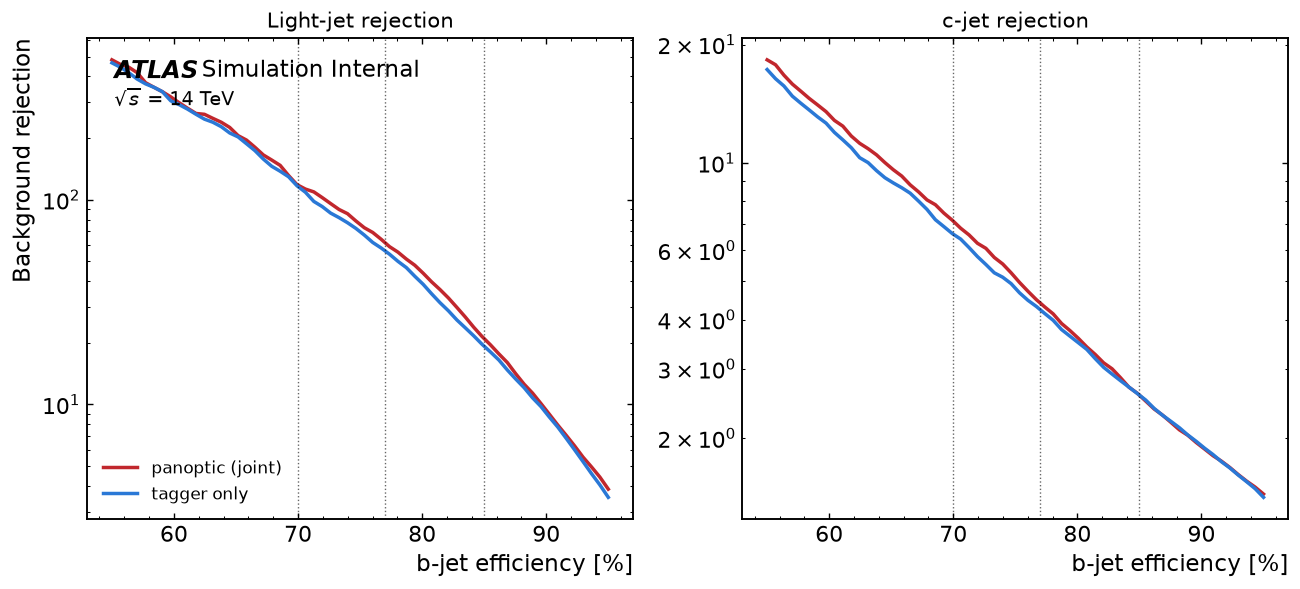
\includegraphics[width=\textwidth]{T2A_rejection_curves.png}
\caption{Background rejection versus $b$-efficiency for light (left) and $c$ jets
(right): the joint model (red) matches or exceeds the dedicated tagger (blue) across
the working range; working points marked.}
\label{fig:rej}
\end{figure}
\begin{figure}[htbp]\centering
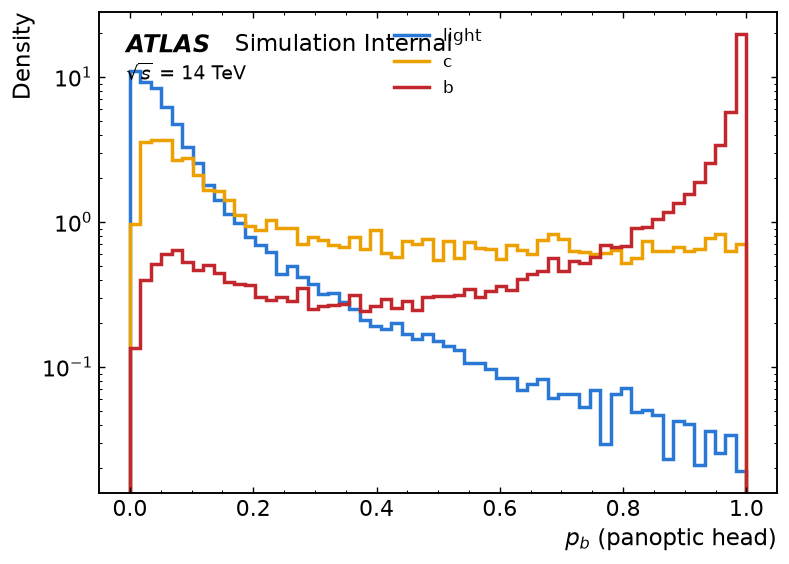
\includegraphics[width=0.6\textwidth]{T2B_scores.png}
\caption{Panoptic $p_b$ by true flavor: clean $b$/light separation with $c$
intermediate, as physics dictates.}
\label{fig:scores}
\end{figure}
\begin{figure}[htbp]\centering
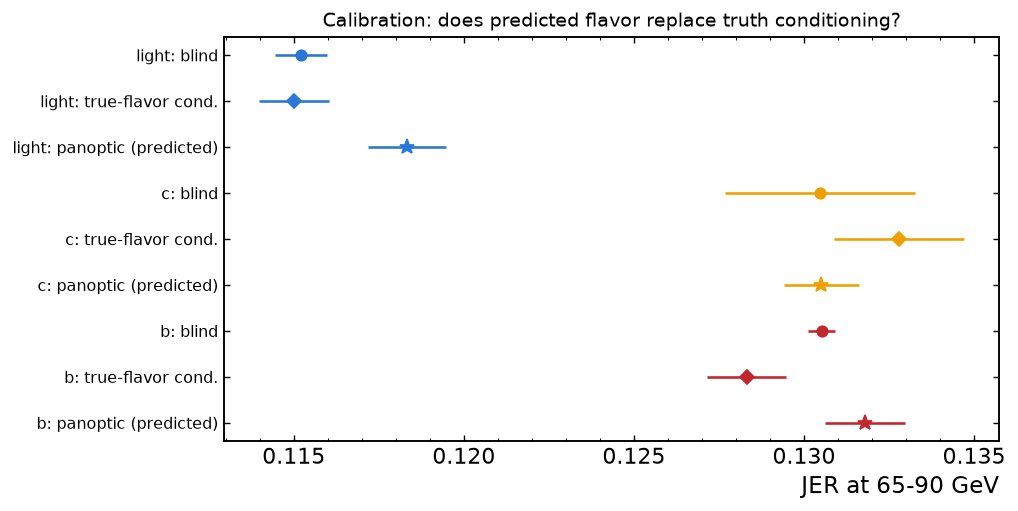
\includegraphics[width=0.7\textwidth]{T2C_calib_compare.png}
\caption{Per-flavor JER at 65--90\,GeV: blind (circles) and truth-conditioned
(diamonds) from Note~02, versus the panoptic model with predicted flavor (stars). The
panoptic model recovers most of the conditioning benefit---and improves charm---%
without truth labels at inference.}
\label{fig:calib}
\end{figure}

Calibration: overall JER@65--90 $=0.126$ versus 0.123 for the truth-conditioned model
of Ref.~\cite{note2} and 0.124 blind; closure RMS 4.3\%. Per flavor (seed 0): light
0.120, $c$ 0.129 (better than truth-conditioned 0.133), $b$ 0.133 (vs 0.128). The
dedicated-tagger run's calibration outputs are untrained by construction and excluded
from comparison.

\section{Conclusions and outlook}
A single panoptic head performs flavor tagging at parity-or-better with a dedicated
tagger while calibrating within ${\sim}2\%$ of the truth-conditioned optimum---the
two tasks share representation, and each supplies what the other needs. Next steps in
the program: event-level missing-$E_\mathrm{T}$ estimation (truth MET derivable from
the neutrino record) and query-based jet finding, extending the panoptic principle
from per-jet to per-event reconstruction.

\begin{thebibliography}{9}
\bibitem{note1} DFM-NOTE-2026-01, \emph{Machine-Learned Jet \pt{} Calibration from
Low-Level Detector Information},
\texttt{notes/DFM-NOTE-2026-01-jet-pt-calibration/}.
\bibitem{note2} DFM-NOTE-2026-02, \emph{Flavor-Dependent Machine-Learned Jet
Calibration}, \texttt{notes/DFM-NOTE-2026-02-flavor-calibration/}.
\end{thebibliography}
\end{document}
